\documentclass[hidelinks,12pt]{report}
\usepackage[utf8]{inputenc}
\usepackage{float}

\usepackage[margin=1.2in]{geometry}
\usepackage[T1]{fontenc}
\usepackage{graphicx}
\usepackage{pdfpages}
\usepackage{mathtools}
\usepackage{hyperref}
\usepackage{mathtools, bm}
\usepackage{amssymb, bm}
\usepackage{indentfirst}
\graphicspath{ {images/} }
%indent
\setlength{\parindent}{1em}
\setlength{\parskip}{1em}
%figures at the begining of page
\makeatletter
\setlength{\@fptop}{0pt}
\makeatother
%for tables
\newcommand{\bigcell}[2]{\begin{tabular}{@{}#1@{}}#2\end{tabular}}


\begin{document}
\begin{center}
\begin{large}
\textbf{Acknowledgment} 
\end{large}\\~\\
\end{center}
\par This project would have not been possible without the collaboration between the CNSMDP  (\textit{"Conservatoire National Supérieur de Musique et de Danse de Paris"}) and the laboratory of IRCCYN (\textit{"Institut de Recherche en Communications et Cybernétique de Nantes
"}). I would like to thank especially Dr. Mathieu Lagrange who has put his trust in me on completing this project, for his guidance all along my internship and his suggestions that helped me achieve the results reported here.\\ I would also like to thank Vincent Lonstanlen, for his guidance on how to use the Matlab toolbox Scatnet, and for his suggestions during the progress of my internship.
\thispagestyle{empty}
\newpage
\tableofcontents
\thispagestyle{empty}
\newpage
\clearpage
\thispagestyle{empty}
\newpage
\listoffigures
\thispagestyle{empty}
\listoftables
\thispagestyle{empty}
\newpage
\clearpage
\setcounter{page}{1}
\noindent




\chapter{Introduction}

\section{Data mining for music}
In a daily basis, a big amount of musical data is being uploaded to the web. This data can take many form, and include a lot of information. Some example of what information can be taken from those data are the genre of the music, the gender of the artist, the lyrics of songs, the instruments being played ...\par
With the increase of those data comes a challenge of identifying and classifying the musical data on the web. Data mining refers to a process of automatically extracting important information from files in a database. In music, data mining has got a lot of attention of the musical and machine learning community in the past years. This paper shows the work done in extracting information related to instruments and playing techniques.

\section{CNSMDP and TICEL Project}
The CNSMDP  (\textit{"Conservatoire National Supérieur de Musique et de Danse de Paris"}) offers a high level training in the domain of music,dance and sound technologies. Placed under the tutelage of the French Ministry of Culture and Communication, the conservatory offers to its 1300 students a cutting edge study programmes. Also, to keep up with the new technologies and help in its advancement, a lot of projects are launched to benefit from the digital advancement in the musical and dance domains. \\
The project TICEL (\textit{"Traité instrumental collaboratif en ligne"}) falls directly in that perspective. It was launched in collaboration between the CNSMDP, "\textit{'Ecole normale supérieure de Paris}" and \textit{"Ecole centrale de Nantes"}. The project was thus supervised by Dr. Mathieu Lagrange at the laboratory of IRCCYN (\textit{"Institut de Recherche en Communications et Cybernétique de Nantes"}) in the city of Nantes. I was asked as part of my final year project to conduct an internship on the project. \par
The purpose of the internship is to study the sounds played by different instruments with different playing techniques. The music samples are thus represented in a space of descriptors that enables the  discrimination between two instruments and their relative playing techniques. This discrimination is done by finding a space where an euclidean distance is maximum for inter-class observations and minimum for intra-class observations. The goodness of fit of the space is evaluated using two ranking metrics: the mean average precision (MAP) and the precision at k (P@k). The study is done on the SOL database that is presented in the next paragraph.  \\ 

\section{The SOL database}
The SOL database is provided as part of the Orchids orchestration system by the team IRCAM. It contains 25119 audio files stored in the 24 bits / 44.1 kHz format. The sounds are played by 16 different instruments which can be subdivided into 32 different classes. There are 498 different combination of instrument with different playing techniques. The database contains three types of instruments varying from strings (Violin, Viola, ...), woodwind (Flute, Oboe...) and Brass (Trumpet, Trombone,...). The techniques of playing on each instruments vary from instrument to another and include techniques such as Aeolian, crescendo, flatterzunge... A full list of instruments and playing techniques is provided in \cite{SOL}.
Figure 2.1 shows the distribution of the SOL database along 6 octaves and one non acoustic class. The biggest part is octave 4 where all the instruments are represented in it (with different proportions).

\begin{figure}[t!]
  
  \centering
	    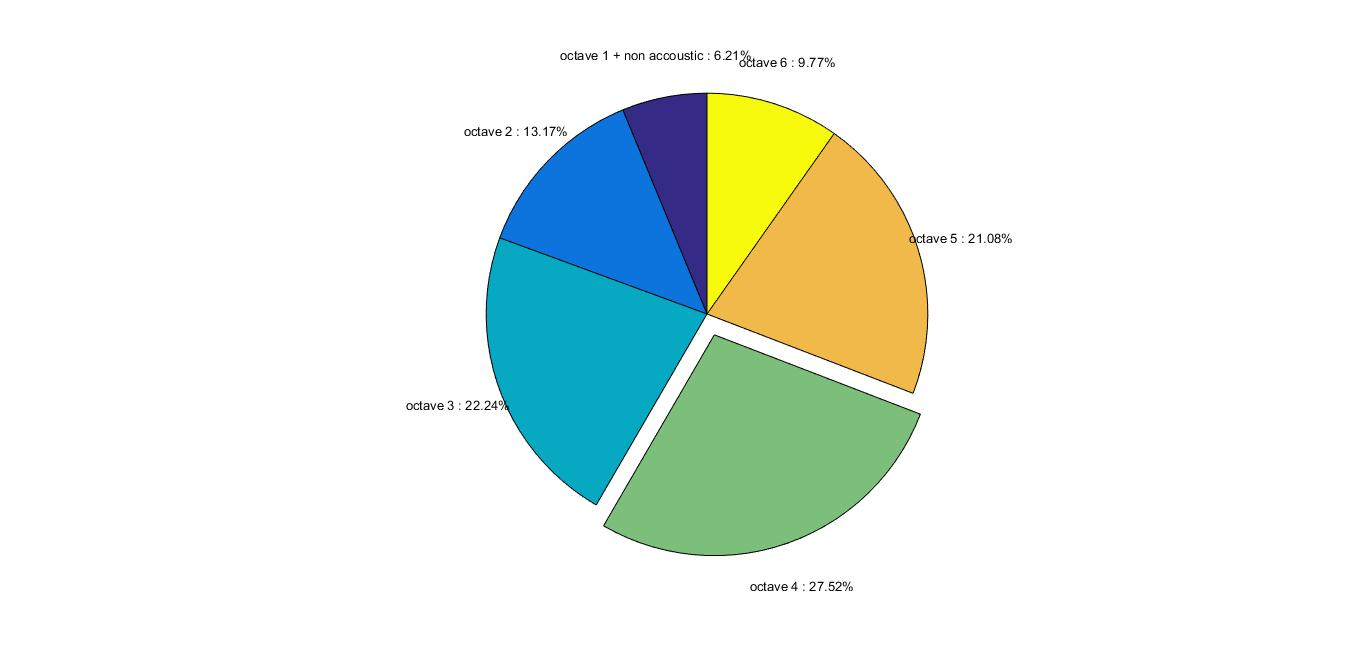
\includegraphics[width=1\textwidth]{byoctave}
    \caption{Musical octave study of sol database}
\end{figure}


\section{Human interpretation and timber}



Before presenting the work done in this internship it is interesting to look on how this discrimination between sounds is naturally done by human.\par
\begin{figure}[t!]
  
  \centering
	    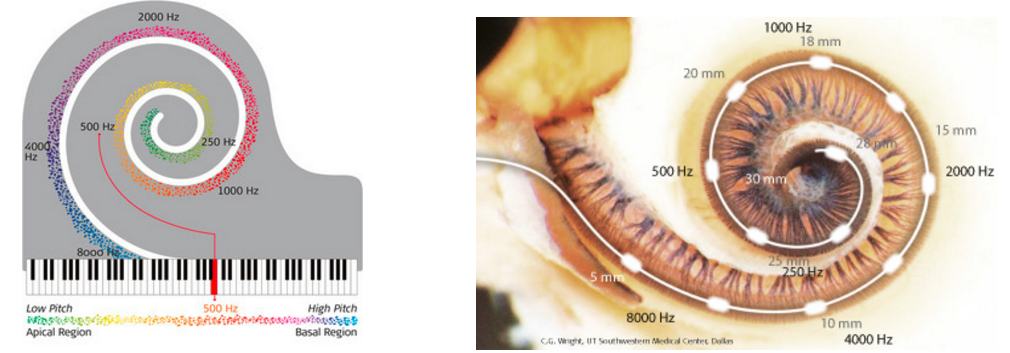
\includegraphics[width=1\textwidth]{cochlear}
    \caption{Scheme of the cochlear taken from medel.com website}
\end{figure}
\subsection{The mechanics of hearing}
Our brain processes sounds by analyzing both the frequency components of those signals and the temporal change of amplitude. To better understand this phenomena, the figure 1 shows a scheme of the cochlea located inside the ear. On the right part of the picture, the figure shows that the cochlea contains hair resonating  at different frequencies. Those small hair will trigger a nerve. this nerve will inform the brain on which frequencies is being heard by the ear. The brain will thus have three information to process, the frequencies, their relative loudness and the time they are being heard. Based on those three information the sound will be constructed, allowing us to
recognize the loudness, pitch and timbre of the sounds we are hearing. Other perception factors can help in recognizing the spacial coordinates   of that sound.

\subsection{The psychology of hearing}

In our daily interaction with our environment, our brain processes the sound that is being heard by the ear. This processing is what gives the sound a meaning .For example, hearing the sound of a train behind us is directly correlated with fear. Another example more relevant to our study, a french person hearing an arabic song will react to it differently from a native person. To fully understand how we interpret sound, the mechanical factors inside the ear are not enough. Just as all the other senses, a psychological aspect should be taken into account to build the whole picture of our interpretation of reality. This aspect can not be explained with equations yet, rather it is better understood with experiences or with functional study of the brain. The last section of this paper will be dealing with one similar problem of understanding the psychology of interpreting instrument sounds.\par 


This report perform studies on the similarity between different audio recordings coming from the same or from different instruments with different playing technique, and since timber by its most general definition is what allows us to experience, the same note played with the same loudness, in a different way for each instrument.\\ Let us first start by talking about  timbre, then present the problem and its proposed solution. 



\section{What do we know about timbre ?}
Since the first explanation of sounds put by Helmholtz in 1863 \cite{H95}, the definition of timbre has changed, especially with the inability of modern day synthesizers to reproduce the same auditory experience of an instrument based on a primal definition of timbre. After a lot of studies done on the subject by physicists, biologists and musicians we have a clear definition of what timbre is not rather than what it really is. For instance, the American National Standard Institute ANSI in the American National Standard on Acoustical Terminology (\textit{ANSI S1.1-1994}) defines timbre as follows :
\begin{quote}
\textit{"Timbre is that attribute of auditory sensation in terms of which a listener can judge that two sounds similarly presented and having the same loudness and pitch are dissimilar." ANSI 1994}
\end{quote}
This definition clearly states that timbre is not related to the loudness, pitch or the duration of the tune being played (or spoken). This being said, There are still many factors that help us distinguish between two notes played with the same loudness, pitch and duration, those factors are considered as part of the structure of timbre. Some example of those factors:
\begin{itemize}
\item The difference in amplitude of the harmonics.
\item Change in harmonics during the attack.
\item The deviation of the harmonics from the perfect $n*f$ location where f is the fundamental note and n is an integer.
\item The vibrato of the note.
\item The sustain and the decay of the note. 
\end{itemize}
The notion of timbre is still an abstract one, thus it will be an obvious step to try to find another solution to solve the problem.
\section{Defining the problem}
To try and achieve the best results, the project was divided into two parts. The first part is based on the true labeling of the data and the second part is based on a ground truth experiment conducted on 78 samples.
\subsection{Ranking against the instrument class and the playing technique}
In the first section of the project, the complete Sol database is studied by dividing it into classes. Three type of classes are studied :
\begin{enumerate}
\item classes of instruments.
\item classes of instruments with variation(with mute, without mute...).
\item classes of instruments with different playing techniques.
\end{enumerate}
In this part, the labeling is taken from the physical nature of the instrument, and no human opinion affects the decision of the labeling. The problem being thus faced is one of discriminating between instruments based on the physical aspect of the instruments or playing techniques. It should be noted that the difficulty of the problem increment with the number of classes. For example, it easier to differentiate between two instruments than between the playing techniques.\\ The anticipated end result is to find the space where the five nearest neighbors to each sample are from the same class.

\subsection{Acoustical description against perceptual judgments}
In the second part of the project, a similarity study was conducted and 32 different subjects. it subject gave labeling based on their interpretation of 78 samples taken from the complete database. This time the labeling is affected by the psychological way each person hear the sound. The similarity between two samples is not only based on the true nature of the sound but also on how each subject interpret the sound.\\ The objective in this section is that the five nearest samples are from the same class based on the average opinion of all the test subjects.

\section{Solving the problem}
In both cases, the first step is to identify the space in which the study of the data should be made and proceed to proper feature extraction. Two ways of looking at the feature extraction problem can be considered: perceptual or taxonomic \cite{P03}. The perceptual approach is motivated by the biological aspect of the problem, and it aims to explain how we hear the sound by finding a space where the descriptors axis explains the notion of timbre. This aspect will not be discussed in this paper, rather the taxonomic approach will be studied. In the taxonomic approach the best feature space is the one that helps in getting the most discrimination between classes.\par
A state of the art study was done on the subject of features extraction for audio samples. Based on that study, two space representations are considered; the first one is the MFCC and the other is the scattering \cite{AM11}. In both cases the highest precision based on the Mean-Average-Precision and Precision-At-5 should be achieved using techniques of data treatment and metric learning. 

\section{The ranking metrics}
\subsection{Computing the distances}
To evaluate the performance of each space, the pair wise euclidean distance between each two instrument samples in that space is computed. For n number of files an n*n symmetric matrix of distances is thus obtained. The 5 smaller distances to each file are extracted. For each file 5 other suggestions are kept. This method is usually used to evaluate search engine. Thus our problem can be looked at as being a search engine based on instrument or playing techniques. A success would be to give 5 suggestions that are from the same class (same instrument or same playing technique).
\subsection{The mean average precision}
The MAP is a single evaluation number of the whole search system performance. This is the most used number in the domain of search systems. In the mean average precision, the mean stands for averaging on the entire different queries results. The average precision or AP stands for the average precision of each query result alone. In brief, for each query, the average precision and then average on the entire query space are computed. Let us now define the average precision.
\subsubsection{Average precision}
To better understand the average precision Let us consider an example  in fig \ref{map}. Let us take the five nearest samples to the yellow sample inside the square. And let us denote By 1 if the other sample is in the same class and 0 if not. the five nearest samples would be evaluated as [1 0 0 1 1]. The precision of each sample is given by the following equation : $$precision=\frac{relevant\  retrieved}{retrieved}$$. The precision of the samples would thus be equal to : $$[1/1 \  1/2 \ 1/3\  2/4\  3/5]=[1 \ 0.5 \   0.33 \ 0.5 \ 0.6]$$\\ the average precision would then be equal to the sum of those samples divided by the number of samples.$$AP=\frac{1+0.5+0.33+0.5+0.6}{5}=0.586$$
\begin{figure}[t!]
  
  \centering
	    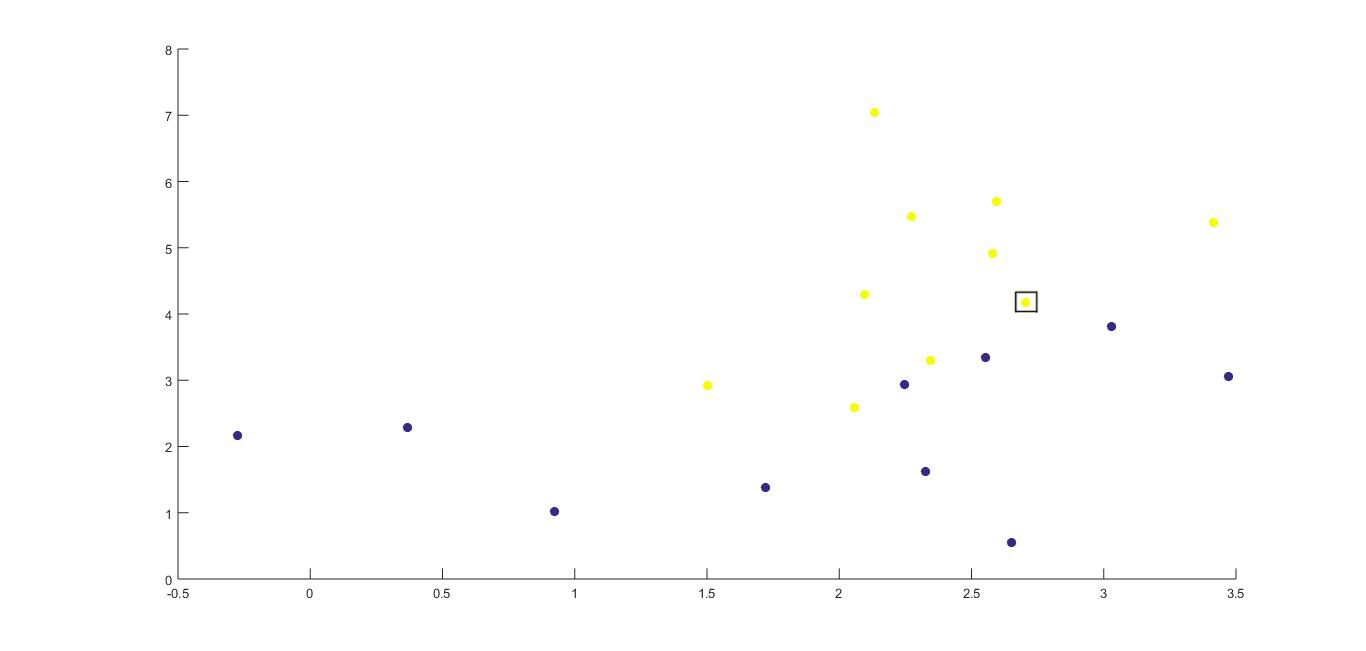
\includegraphics[width=1\textwidth]{fig1.jpg}
    \caption{Example to demonstrate the average precision}
    \label{map}
    \label{fig:toto}
\end{figure}
The same computation will be done for all the samples in the space. and at the end we sum all the AP and divide them by the number of samples to obtain the mean average precision. As we can see the mean average precision put more weight on having the first result as a relevant sample(same class) than the second result and so on.
\subsection{The precision at k}
The precision at k is another ranking metric that is used to evaluate the result of a search query. As  its name indicates we are only interested of the precision at a given rank k. in our example we take the precision at 5 as a metric to evaluate the data. This metric is very useful to indicate if the user will get a relevant document in the 5 first result. A major disadvantage of this metric is that it does not take into consideration the position of that file in the result, meaning that, for a certain search query, if we have n out 5 relevant files it doesn't matter if the first one is relevant result or not. The precision at k is the average of all the precision of each sample alone.









\chapter{Ranking against the instrument class and the playing technique}
\section{Clustering the samples}

In the first part of the study, the following ranking problem was studied. 25119 musical extraction are provided of different solo instruments played with different techniques. Those samples are clustered in three different ways: 
\begin{enumerate}
\item \textbf{ 16 classes of instruments.}\\
In the first labeling type the samples are classified based on the instruments they are played with. Since the database provided contains 16 different instruments, the samples are divided in 16 different clusters.
\item \textbf{32 classes of instruments with variation.}\\
To add some complexity to the instrument clustering and to further test the stability of the code, an additional variation to the instruments clustering is considered. So for example, a sample played without mute is given different label than a sample played by the same instrument with mute.
\item \textbf{498 classes of instrument with different playing techniques.}
The last clustering and the most complex ranking problem to solve, is considering that two samples played with different techniques will have different labels even if they are being played by the same instrument. Thus there is 498 different labels in this clustering.\\

\end{enumerate}
\section{Experimental procedure}
The experimental procedure is composed of two parts. The first one computes the features based on one of the two representations: MFCC or scattering (with different parameters). In the second part the ranking metrics are computed before and after processing the data in the feature space.\par
In the first part, the use of the two representations is done as follows : using a fixed length window of calculation a certain number of temporal features are obtained based on the length of the signal. Then, by averaging along the time axis, only one vector of features by audio file is left.\\ 
For the second step, the distance computation is done using pairwise Euclidean distance measure. Many form of processing in the feature space are tested and only the one that proves efficient is shown here and presented in further details in later sections:
\begin{itemize}
\item Standardization.
\item High or low variance filtering.
\item Projecting into symmetrical data by whitening.
\item Large Margin Nearest Neighbor.\cite{W09}\\
\end{itemize}

The evolution of the data is done in the Euclidean space after preprocessing the data. The two ranking metrics, MAP and P@5, are used for the evaluation.


\begin{figure}[t!]
  
  \centering
	    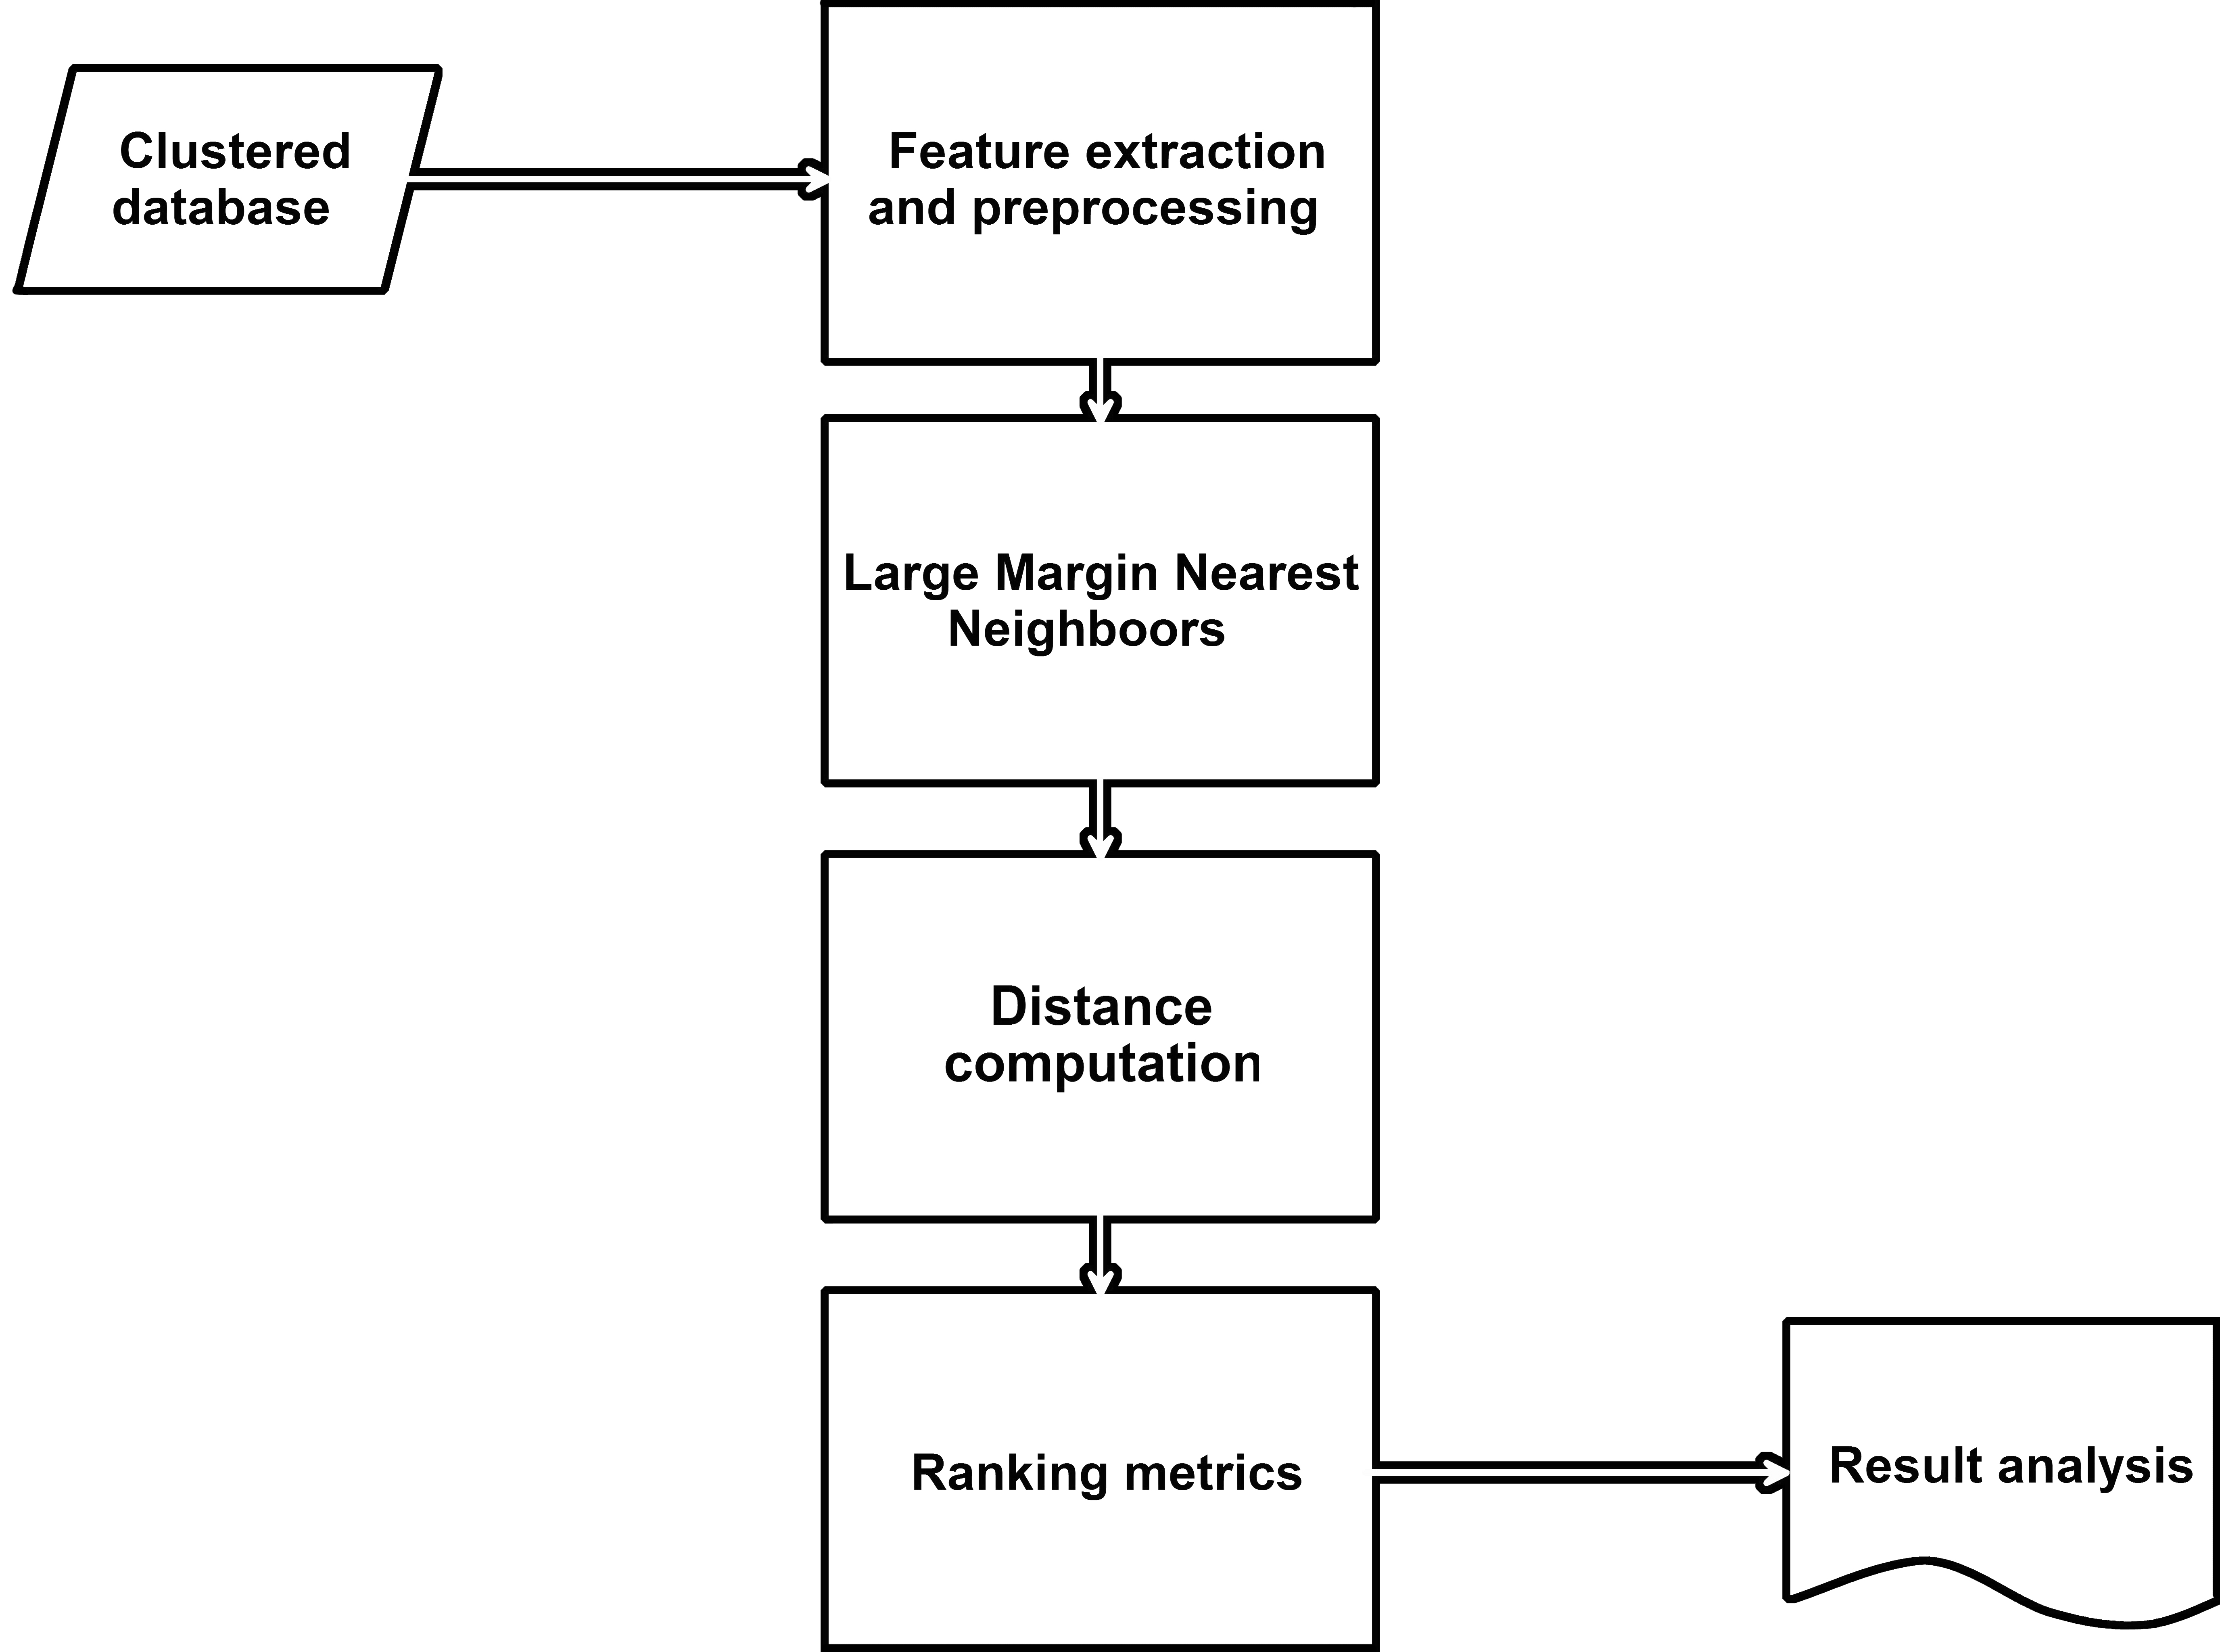
\includegraphics[width=1\textwidth]{experimental_procedure}
    \caption{Experimental procedure }
    \label{experiment}
\end{figure}
The following sections follows the same scheme presented in figure \ref{experiment}. First the feature extraction procedure is presented, following are the methods of processing in the feature space. At the end, The performance is analyzed using the distance computation and ranking metrics.

\section{Feature extraction}
In this section the two methods of feature extraction studied in this report are presented alongside the motivation and the algorithm of computation. First the Mel Frequency Cepstral Coefficients are presented followed by the scattering representation. 
\subsection{Mel Frequency Cepstral Coefficients MFCC}
The MFCC (Mel Frequency Cepstral Coefficients)  became famous with the rise of speech recognition systems. The MFCC are able to mcast a spoken stream in a compact and meaningful space. Those coefficients contains most of the information needed for processing spoken audio streams. They are still found in most of the audio processing applications. In the musical domain MFCC has been widely used for music genre classification.\\ The biggest limitation of the MFCC, as we will see in details, is its inability to encode large time scale variation.

\subsubsection{Algorithm and motivation}
\begin{figure}[t!]
  
  \centering
	    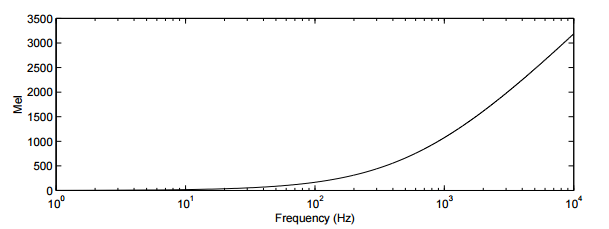
\includegraphics[width=0.7\textwidth]{melscale}
    \caption{Mel scale }
    \label{mel}
\end{figure}
The extraction of the MFCC features is divided into 5 steps as presented in figure \ref{mfcc}. In this part, Each step is presented along with the motivation and the limitation it provides.
\begin{figure}[t!]
  
  \centering
	    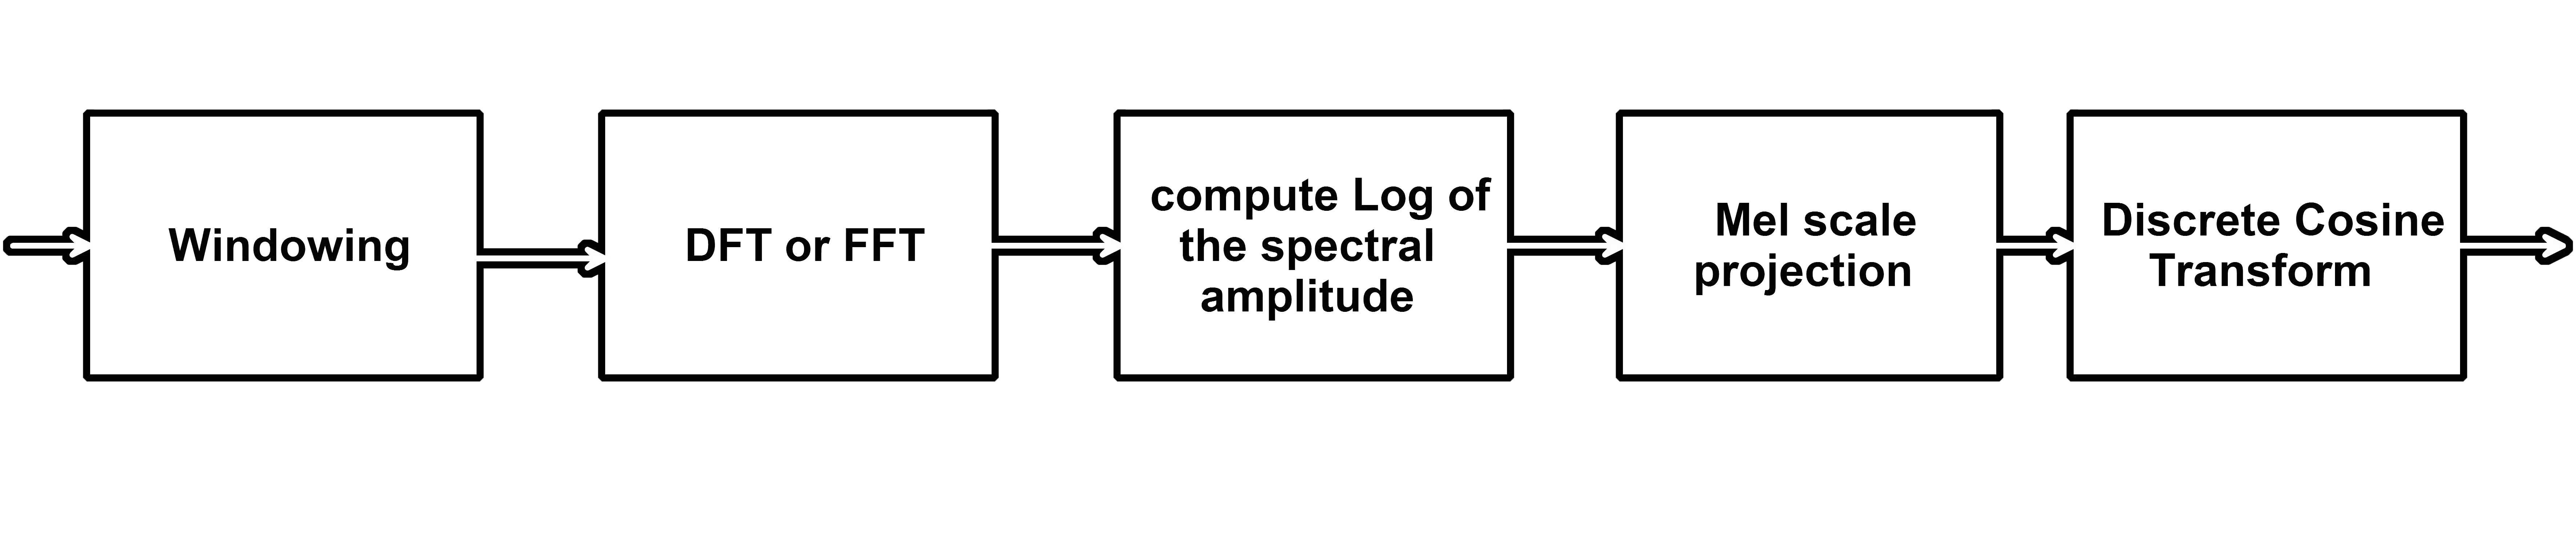
\includegraphics[width=1\textwidth]{MFCC2}
    \caption{Procedure of MFCC feature extraction }
    \label{mfcc}
\end{figure}
\begin{enumerate}
\item \textbf{Frame division} \\
The first step is to divide the waveform into equal spaced frames in the time domain. The split is obtained by applying a windowing function at fixed time intervals. This step is motivated by the fact that audio signals (music and speech) can be considered a statistically stationary for a short period of time. The limitation of this step is related to the length of the windowing function. It is proven that the best results are obtained for a window function length between 25 and 40ms. The longer the frame the bigger the variation of the signal in each frame and this will lead to a loss of information. 

\item \textbf{DFT or FFT computation\\}
The discrete Fourier transform (or fast Fourier transform) is used to project from the time domain to the frequency domain. By using the Fourier transform the amplitude of the spectrum is taken inducing a loss of knowledge on the phase. The motivation of computing the MFCC, is that the information provided to the brain by the cochlear is the amplitude of the frequencies(1.3.1).
\item \textbf{LOG of amplitude spectrum computation}\\
The log of the spectrum amplitude obtained by the Fourier transform is taken. This step is motivated by the human perception of the sound loudness. The loudness of the sound is perceived by human in a logarithmic way : 8 time more energy should be put into a sound loudness to double the hearing experience. 
\item \textbf{Mel scale projection}
This step is done to reduce the space and smooth the spectrum by applying a mapping from the log amplitude spectrum to the Mel frequency scale. This mapping is logarithmic for high frequencies(higher than 1KHZ) and linear for low frequencies(below 1KHZ). The scale is motivated by the fact that human do not perceive pitch in a linear way. The mapping allow human to reduce the space to n features space, where n can vary up to 40.
\item \textbf{DCT computation}
Now 40 highly correlated features are left and most of them containing unnecessary information. To achieve the decorrelation and to extract the interesting features a Discrete Cosine Transform is applied and only the first 12 of the 27 features are kept. 
\end{enumerate}
\subsubsection{MFCC parameter choice}
Before applying preprocessing techniques to the MFCC, a tuning on the values of different parameters should be tested. the default factors for the MFCC were proven to be the best.

The results are shown in the table below. Divided into three parts with the number of class varying from 16,32 to 498. Two variations of the mfcc are shown with the first one is by taking 12 features out of the 27 and the other is with taking all the 27 features. The last one is by taking the features in the mel space without applying the DCT(40 features).\\

\begin{table} [H]
\begin{center} 
\ 
 \setlength{\tabcolsep}{.16667em} 
\begin{tabular}{ | l | l | l | }
\hline 
features & map & pat5 \\
\hline
\hline
16 classes of instruments    \\ 
\hline 
mfcc 12/27  & 22.66 & 85.93  \\ 

mfcc 27/27  & 19.72 & 85.24  \\ 

mel &  16.48 & 62.90 \\

 \hline 32 classes of instruments with variation  \\ \hline
mfcc 12/27  & 20.84 & 83.98  \\ 
 
mfcc 27/27 & 17.87 & 82.85  \\ 

mel  & 14.72 & 60.26  \\ \hline

498 classes of playing techniques   \\ \hline

mfcc  & 8.24 & 43.95 \\ 

mfcc 27/27  & 8.85 & 43.96 \\
mel  & 5.74 & 32.90  \\ \hline
\end{tabular} 
\end{center} 
\caption{Results of the study performed on the MFCC features. Labels taken as 16 class of instruments, 32 classes of instruments with variation, 498 classes of techniques of play} 
\label{you} 
\end{table} 

The best results were proven to be by taking 12 out of the 27 MFCC coefficients, this is due to the fact that those coefficients better represent the physical aspect of the instruments used.

\subsubsection{MFCC features preprocessing}
When dealing with a big space of data, Usually a preprocessing technique should be applied before proceeding to use a learning algorithm. This usually proves to be efficient, and there are  different techniques of normalization that can be tested for example :   The effect of preprocessing the MFCC features was tested using the standardization technique.\\
\textbf{Feature standardization :}
In feature standardization, each feature is taken independently and treated in the following way : \\
for each dimension,
\begin{itemize}
\item Compute the mean.
\item Substract the resulting mean.
\item Compute the standard deviation.
\item Divide by the standard deviation.
\end{itemize}
This technique is widely used as a preprocessing for MFCC, since it removes the effect of the DC component that overshadows the space. The result of applying the standardization is shown in the table below.
\begin{table}[H] 
\begin{center} 
\ 
 \setlength{\tabcolsep}{.16667em} 
\begin{tabular}{|l|l|l|} 
\hline
features & map & pat5  \\ 
\hline
\hline
16 classes of instruments    \\ 
\hline 
raw & 22.66 & 85.93  \\ 
standardize & 24.22 & 86.89  \\  

 \hline
 32 classes of instruments with variation \\

\hline 
raw & 20.84 & 83.98 \\ 
standardize & 22.29 & 85.12  \\ 


\hline 
498 classes of playing techniques \\
\hline
raw & 8.24 & 43.95  \\ 
standardize & 8.78 & 45.19  \\ \hline 
\end{tabular} 
\end{center} 
\caption{Comparison between MFCC before and after standardization for the 16 classes of instruments, 32 classes of instruments with variation, 498 classes of playing techniques} 
\label{me} 
\end{table}



As it is shown in the tables, the results indicate that standardization yields to a slight performance while performed in the MFCC feature space. This improvement is due to the fact that some of the features in the MFCC will be highly weighted and affects the other features. By standardizing this effect will be reduced. Since the space is compact, and the MFCC itself contains preprocessing techniques such as decorrelation the improvement is in the order of 1\%.

\subsection{The Scattering transform}
\begin{figure}[t!]
  
  \centering
	    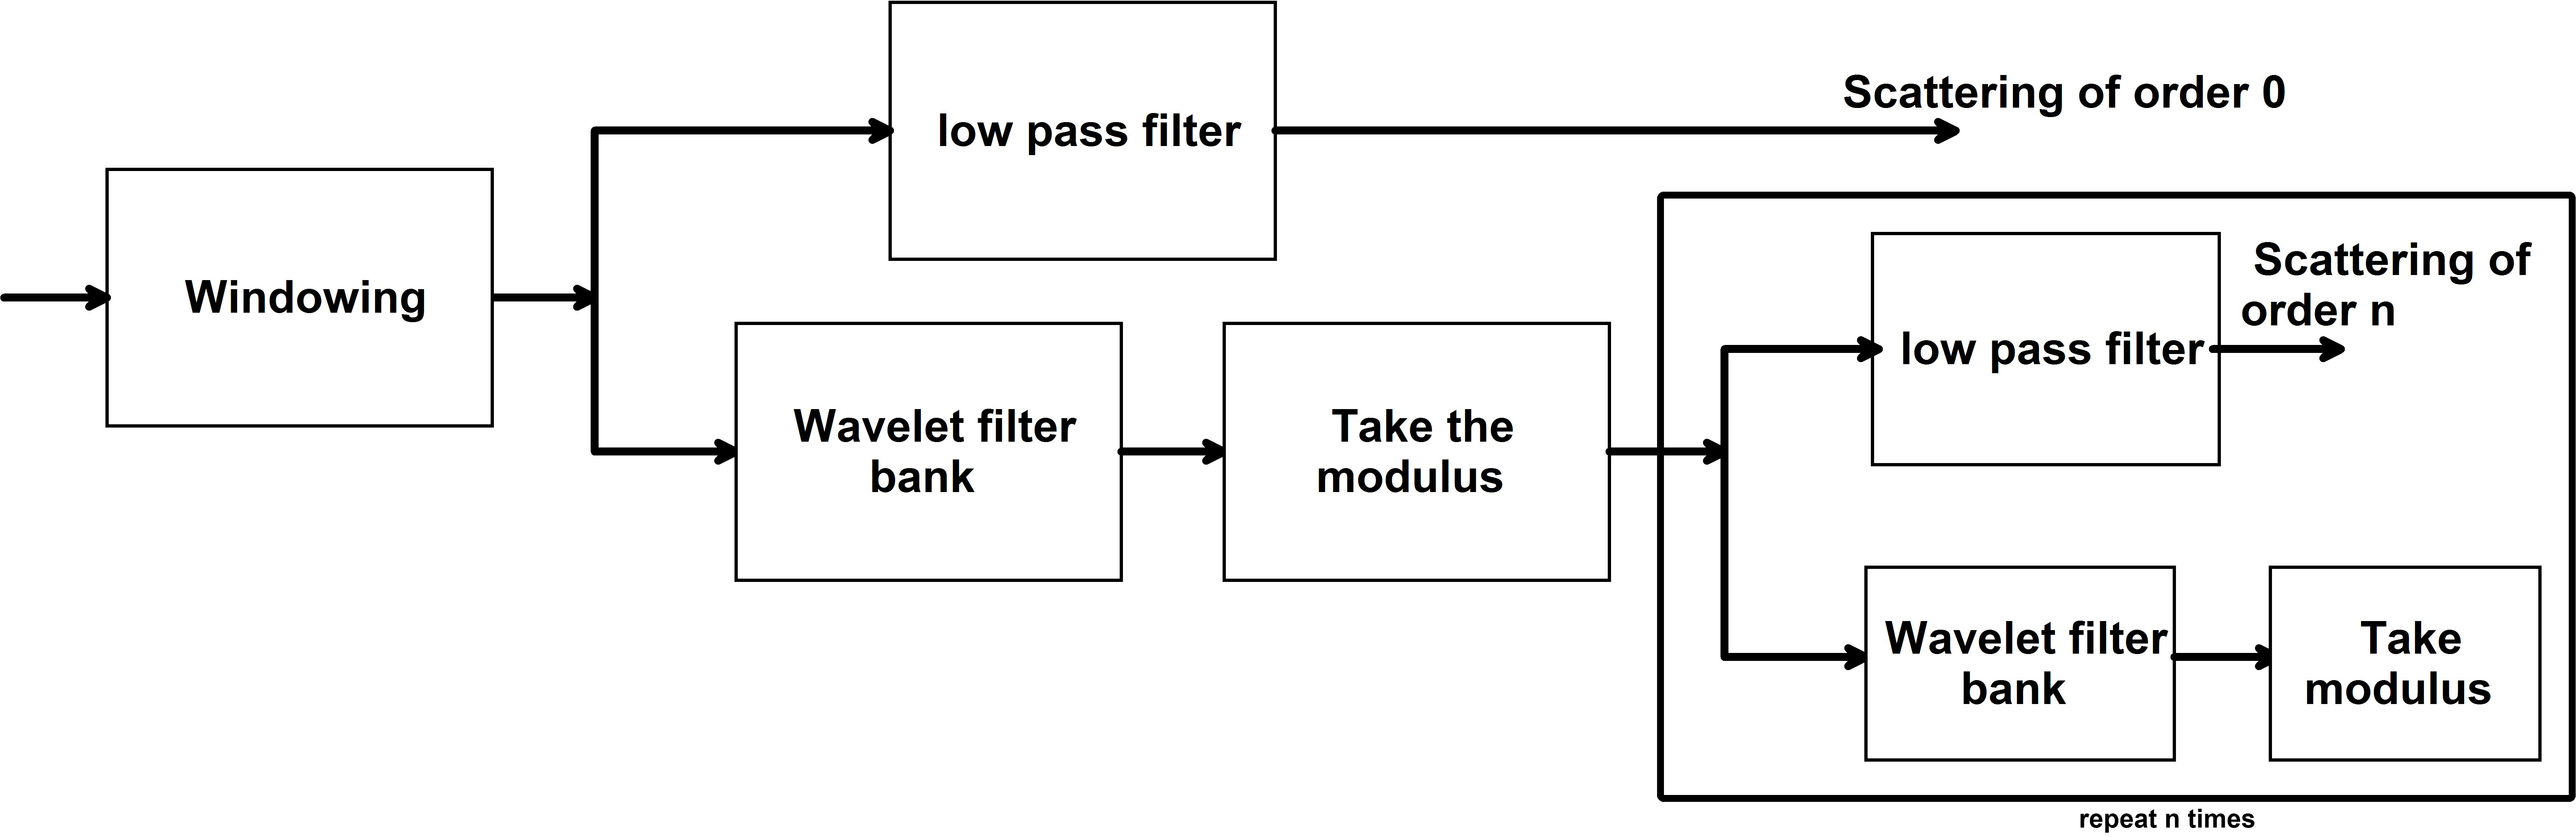
\includegraphics[width=1\textwidth]{scattering}
    \caption{Scheme of the scattering transform procedure }
    \label{scat}
\end{figure}
The second feature extraction method that was studied is the scattering transform. This method achieves signal decomposition using multiple wavelet transform alongside modulus operators. Figure \ref{scat} shows a scheme of how the procedure of extracting the scattering coefficients works.\par This method first proposed by Stephan Mallat in \cite{M10} is relatively new. A lot of research are being made on its application in different domains such as image and audio. In this paper a study on its effectiveness for music classification problems is presented.


\begin{enumerate}
\item First divide the audio samples into frames by using a windowing function. Those windows can vary from multiples of 10 milliseconds to the order of multiples of 100 milliseconds.  
\item Apply to the frames a low pass filter. The output of that filter will be the scattering of order n.
\item Apply to the frames a wavelet filter bank. Take the modulus of the output and replace the frames with the output of this step. 
\item Repeat the step 2 and 3 n times. For audio signals scattering of order 2 is enough to represent the data.
\end{enumerate}
\subsubsection{Reducing variance of the representation}
Audio signals contains information that does not alter the perception of sounds by human. And for tasks such as instrument identification, those information are not important. Such information are : 
\begin{itemize}
\item Translating an audio signal in time will not alter the perception of this sound by humans. Audio signals perception are thus largely time invariant.Indded , discarding the information of time location will not alter the identification of instruments or playing techniques. The representation $\Phi$ will thus have the following property $\Phi(x(t-c))=Phi(x(t))$.
\item Other information that can be discarded are the one related to time warping. Time warping can be considered as shifting the signal by a factor that is time dependent. Audio signals are invariant to small scale time warping. What is needed from the representation is not to be time warping invariant $\Phi (x(t-c(t)))=\Phi(x(t))$ rather to be stable to time warping. This can be seen as a lipschitz continuity condition : $$||\Phi (x(t-c(t)))-\Phi(x(t))|| \leq C||x||||c'||_{\infty}$$
\end{itemize}
The scattering transform is based on a wavelet transform. To better understand how the time shifting and stability to deformation are obtained, let us look at each of the figure \ref{scat} block alone.\par
\textbf{Low pass filter :}
To achieve stability to time shifting, an average in time is applied. This average is achieved by applying a low pass filter. At the first step all the information is lost by this low pass filter, and the result is 0 for scattering of order 0. This same averaging will be applied again before the output of each order to insure time invariance.\par
\textbf{Wavelet filter bank:}
Since a lot of the information is lost in the low pass filter, A series of high pass filters is applied to encode the lost information. To ensure stability to time warping, The high pass filters used are wavelet functions. The use of wavelet is motivated by the fact that at low frequency they have high frequency resolution and at high frequency the have low frequency resolution. This will guarantee overlapping at high frequencies between a signal warped in time and a signal not warped.\par
\textbf{Take the modulus}
By applying a low pass filter again to the output of the high pass filters, again an average of 0 is obtained. To avoid this, a non linearity should be introduced. In the scattering transform, the best non linearity to be considered is by taking the modulus.\par
\textbf{Cascading}
At each step, only the output of the low pass filter is taken. This means that at each step, a loss of high frequency information is forced. To obtain those information again, a cascade High pass filter and low pass filter is done until the loss of information is not significant anymore. To further demonstrate the importance of second order coefficients the following examples is discussed.\par
\begin{figure}[t!]
  
  \centering
	    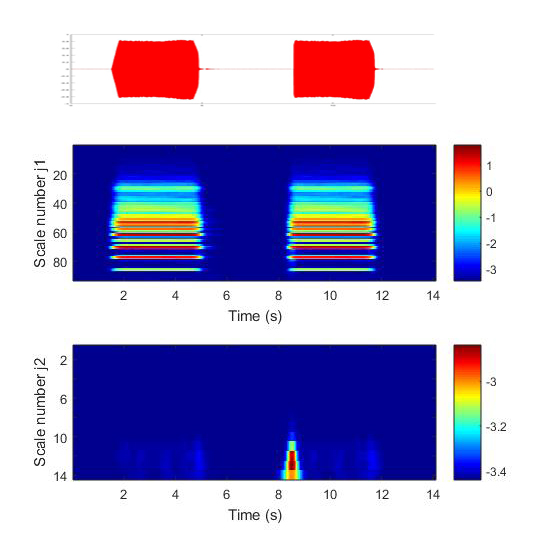
\includegraphics[width=0.6\textwidth]{att}
    \caption{[a.] Variation of amplitude in time of two samples one with smooth attack and the second one with sharp attack. [b.] scattering of order 1 of both signals [c.] scattering of order 2 of both signals }
    \label{attack}
\end{figure}
\subsubsection{Examples presenting the importance of second order}
In the figure \ref{attack} two audio samples are presented of an accordion playing the note A3. The first sample is with a soft attack and the second one is with a sharp attack. Since in the first order coefficient, the resolution of high frequency is low, no information related to the attack can be found easily and the two samples can be confused. \\
By looking at one of the second order coefficients corresponding to one of the high frequencies. The attack can be clearly found. And the difference between the two samples can be easily done.\par
In the figure \ref{vib} the same analysis can  be made. This time The first sample present an audio without vibrato, while the other one present the same audio with vibrato. Since the first order coefficients does not have high resolution for high frequencies, the frequency of the vibrato is lost. By taking the second coefficient of one of the first order feature, the frequency of the vibrato is clearly visible as a frequency not varying in time.
\begin{figure}[t!]
  
  \centering
	    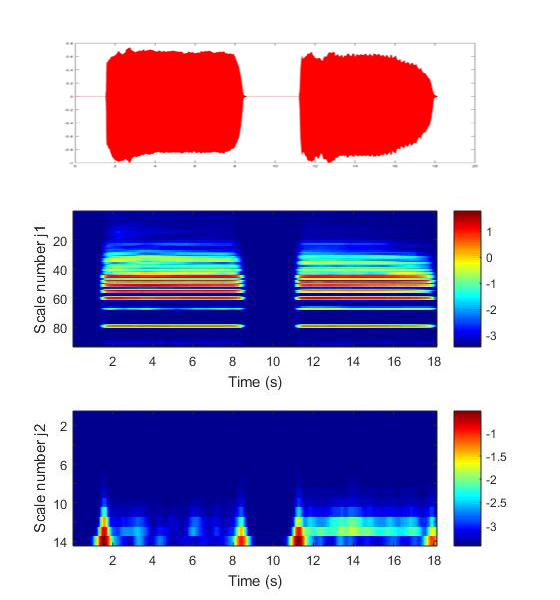
\includegraphics[width=0.6\textwidth]{vib}
    \caption{[a.] Variation of amplitude in time of two samples one without vibrato and the second one with vibrato. [b.] scattering of order 1 of both signals [c.] scattering of order 2 of both signals }
    \label{vib}
\end{figure}
\subsubsection{Results of varying the length of the windowing function T}
The impact of taking smaller window time on the output of the ranking metrics is tested. The test was performed on the 16,32 and 498 labeling variations. The results are given in the following table.
\begin{table} [H]
\begin{center} 
\ 
 \setlength{\tabcolsep}{.16667em} 
\begin{tabular}{ | l | l | l | l | l |}

features  & map & pat5  \\ 
\hline 
\hline
16 classes of instruments\\
\hline
scattering T=25ms & 18.07 & 72.79  \\ 
 
scattering T=128ms  & 16.79 & 70.47  \\ 

scattering T=250ms  & 16.49 & 70.40  \\ \hline
32 classes of instruments with variation\\
\hline
scattering T=25ms  & 16.29 & 70.17  \\ 

scattering T=128ms  & 15.18 & 67.21  \\ 

scattering T=250ms  & 14.89 & 67.05  \\ \hline
498 classes of playing techniques \\
\hline
scattering T=25ms   &  7.79 & 40.17  \\ 

scattering T=128ms  &  6.66 & 37.38 \\ 

scattering T=250ms  &  6.46 & 37.07 \\ 

\end{tabular} 
\end{center} 
\caption{Table comparing the results of applying metric ranking to different window length for the scattering transform.} 
\label{you} 
\end{table}

As presented in the tables, the bigger the windowing time the lower the precision. This is due to the fact that the scattering will be discarding information related to the small time variation. In the next part, the effect of preprocessing on the biggest windowing time is presented.

\subsubsection{Preprocessing the scattering features}
As for the MFCC, the normalization that was tested on the scattering features is the standardization. Another type of preprocessing was applied, that will be referred to as std and median method.\par
\textbf{Std and median method :} The scattering features present a lot of variability in its factors, with some of the factors being irrelevant to the process. To remove those factors and reduce the space, a study of variance should be done. The variance of each feature alone is computed, and sorted by growing values. The accumulated sum is then computed and either the high or the low variances will be discarded. In both cases an improvement was noticed but the best result was achieved with only leaving 83\% of the high variances. This is the std part of the method. \\
The second part is to divide by the vector of median (the median of each feature is computed alone). The feature space is then divided by the median. This will make the distribution of the features symmetrical and close to Gaussian.\\
The effect of the standardization and the std and median method is represented in the table below.

\begin{table} [H]
\begin{center} 
\ 
 \setlength{\tabcolsep}{.16667em} 
\begin{tabular}{ | l | l | l | l | l |}
features & map & pat5  \\ 
\hline 
16 classes of instruments\\
\hline

raw & 16.49 & 70.40  \\ 
standarize & 19.31 & 78.98 \\ 
stdandmedian & 30.43 & 93.21 \\ \hline
 32 classes of instruments \\ 
 \hline
 

 raw & 14.89 & 67.05 \\ 
standarize & 17.52 & 75.13  \\ 
stdandmedian & 27.66 & 90.24  \\ 
\hline
 498 classes of playing techniques \\
 \hline

raw &  6.46 & 37.07  \\ 
standarize & 10.69 & 47.01  \\ 
stdandmedian & 18.59 & 55.44  \\ 
\end{tabular} 
\end{center} 
\caption{Table comparing the results of applying metric ranking to different technique of preprocessing on a scattering with T=250ms considering 16 class of instruments} 
\label{you} 
\end{table}






For the scattering, the preprocessing technique that will be taken into account is the std and median. By considering the table, applying the std and median technique is proved to be beneficial. It is to be noted that the std and median can not be applied to the MFCC since the coefficients taken are already in a very compact space(space of 12 features). \par

In the next chapter, we shall see the results of applying the feature extraction on the ground truth labeling problem.


\chapter{Optimizing an acoustical representation against perceptual judgments}
\section{Introduction}

In this second part of the study, 78 samples are selected from the SOL database and labeled using a perceptual study performed with 32 subjects. Each subject gives different labels based on her/his opinion on which two samples are similar or not. \par
\begin{enumerate}
\item \textbf{Feature extraction} \par
In this part, the same feature extraction method is applied to the samples. The MFCC is extracted and then the standardization is applied. For the scattering, the features are extracted and then the std and median method of preprocessing is applied.




\item \textbf{The metric ranking} \par
To start the study of this method, the two ranking metrics used in the first part should be generalized. The new MAP and P@5 that are used are obtained in the following way :
 \begin{itemize}
\item Compute the metric ranking for each label provided by each subject.
\item Compute the average of the ranking metrics over the 32 set of labels corresponding to each subject.
\end{itemize}

\item \textbf{Results.}

\begin{table}[H]
\begin{center} 
\ 
 \setlength{\tabcolsep}{.16667em} 
\begin{tabular}{ | l | l | l | l | l | l | l |} 
\hline
features & MAP & P@5 \\ 
\hline 
mfcc &  50.74  & 55.66 \\ 
scattering & 40.17 & 44.01  \\ 
mfcc all pitch & 34.96 & 81.27 \\
scattering all pitch & 30.00 & 52.39\\
\hline
\end{tabular} 
\end{center} 
\caption{Results of applying the MFCC and the scattering to the perpectual mapping.} 
\label{ground truth} 
\end{table}
\end{enumerate}

The table shows the results of the ranking metrics applied to the features extracted using the MFCC and the scattering. The MFCC outperforms the scattering even with the preprocessing applied.

\section{Metric learning}

In the first part of the study, the problem was treated without the need of methods of learning. In this part however, the problem is more complicated as labelings are established for each subject differently  based on how she/he experiences those sounds. The problem is to find a space that is not just representative to the physical aspect of the sound but that takes into account the opinion of different subjects. This problem would be very complicated to solve without considering techniques of learning. 


\subsection{K-NN vs search query}
For each query, the space of interest are the closest five samples. This evaluation indicates that beyond those 5 samples, there is no change of precision based on the accuracy of those samples. Thus the evaluation of a search query is highly related to the k nearest neighbors classification.\\
In a k nearest neighbors classification, the euclidean distance is computed between each new sample and the entire samples of the space. For each new sample, a decision is made based on the classes of the the five nearest neighbors. If the majority of the nearest neighbors correspond to a certain class, the new sample will be assigned this class.\\
In both cases (K-NN and search query), an ideal case is that the k nearest neighbor of each sample corresponds to the real class of that sample. However in the K-NN classifier, it is enough to have the majority of the samples assigned with the exact class of the sample where in the search query it is needed to have the k first results from the same class of the search query.\par
The LMNN short for "Large Margin Nearest Neighbor" is a supervised learning method applied to the features space.It is designed to optimize the K-NN classification problem by reprjocting into a space of same dimension by altering the descriptors vectors. Its concept however is well suited for the problem of search query addressed in this paper.


\subsection{Large Margin Nearest Neighbors}
\begin{figure}[t!]
  
  \centering
	    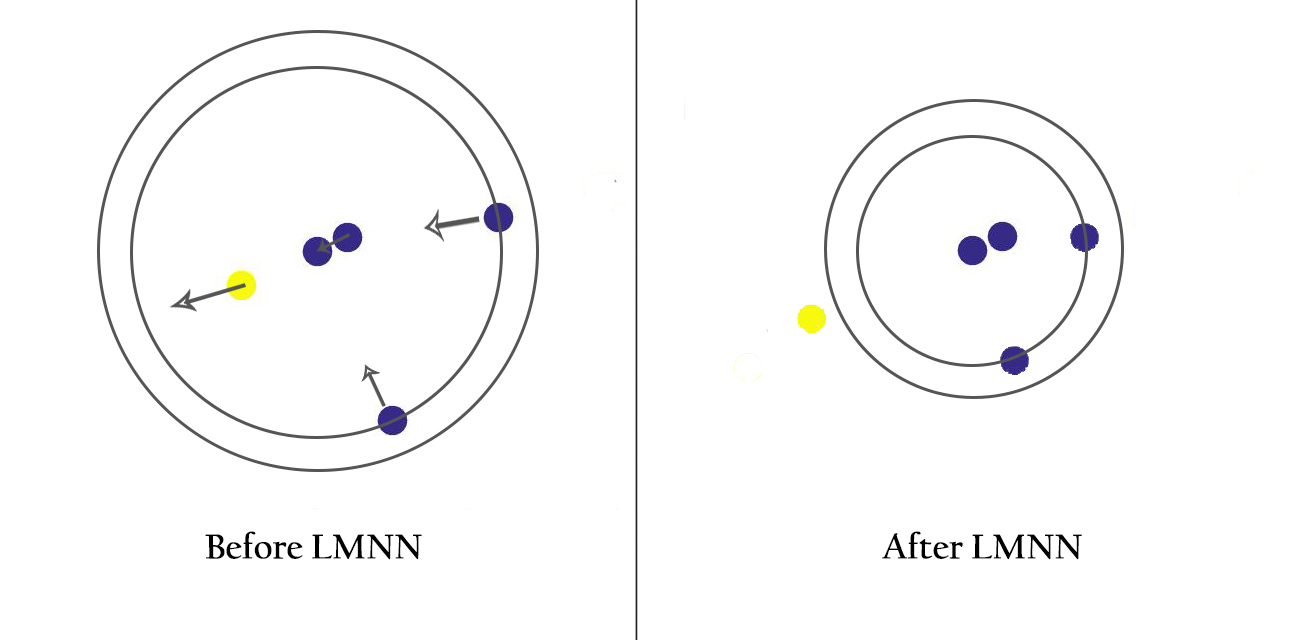
\includegraphics[width=1\textwidth]{lmnn}
    \caption{An example showing the motivation behind the use of the LMNN}
    \label{LMNN}
\end{figure}
The learning technique that is considered in this paper is the large margin nearest neighbors \cite{W09}. In the LMNN the ideal space would be one where each observation has the same class of its K nearest neighbors. This is done in the following way :
\begin{itemize}
\item Compute the pair wise Euclidean distance of the space.
\item Attract the K nearest neighbors corresponding to the same class(Shrink the distance between the observation and the k nearest corresponding to the same class).
\item Set a margin based on the farthest nearest neighbor from the same class.
\item Push all observations from different classes outside this margin (expand the distance between the observation and other samples that violate the margin.)
\end{itemize}
To better understand this idea, let us have a look at the following example in figure \ref{LMNN}. Consider a space of five samples that are divided in two classes. The blue class corresponds to samples played by a violin and the yellow class corresponds to samples played by a guitar. Let us focus on the effect of applying LMNN on the blue sample at the center. The settings of the LMNN will be tuned to a problem of three nearest neighbors classification. As showed in the first part of the figure \ref{LMNN}  that the three nearest neighbors to the blue sample in the middle are as follows : [Violin, Guitar, Violin]. The LMNN algorithm will thus aim to attract the two other samples that correspond to the violin class. To ensure that the guitar will not be one of the nearest neighbors of that sample a margin will be set and the yellow sample should be pushed outside the margin. If the LMNN is applied with success the result will be similar to the second part of the figure \ref{LMNN}. The same process will be applied to each sample of the space.
\subsubsection{Learning a Mahalanobis distance}
To perform the process explained above, the LMNN uses a projection of the space by computing a Mahalanobis distance. A Mahalanobis distance is defined as follows  : $$D_\textbf{M}(\vec{x_i},\vec{x_j})=(\vec{x_i}-\vec{x_j})^T\textbf{M}(\vec{x_i}-\vec{x_j})$$
By considering M as  a positive semidefinite matrix M can be decomposed as follows : $$M=L^TL$$. Thus the Mahalanobis distance can be looked at as being a projection from an euclidean space to another euclidean space using the operator L : $$D_\textbf{L}(\vec{x_i},\vec{x_j})=||\textbf{L}(\vec{x_i}-\vec{x_j})||$$. By using this projection, the same process can be applied to obtain the ranking metrics (MAP and P@5).
\subsubsection{The Model}
 The model to solve this distance learning problem is based on three different optimization problems : \begin{enumerate}
\item Mahalanobis metric for clustering(MMC). \cite{X02}
\item Pseudometric Online Learning Algorithm(POLA) . \cite{S04}
\item Neighborhood Component Analysis(NCA). \cite{G05}
\end{enumerate}
The model formulates the parameter estimation as a convex optimization over the space of positive semidefinite matrices similar to the MMC. The margin by which the classifier is accurate for labeled examples will be maximized similar to POLA. And it is build to learn a Mahalanobis distance for optimization of K-NN classifier accuracy similar to the NCA. 
\subsubsection{The loss function}
The end result of applying LMNN would be to efficiently attract the k nearest neighbors and push impostors outside a certain margin. This formulations leads to a two termed loss function. The penalization is defined as follows : \begin{enumerate}\item Impose penalty on large distances between each sample and the k nearest neighbors with the same class label.
\item Impose penalty on small distances between each sample and samples corresponding to different classes.
\end{enumerate}
Before presenting the equations of the two terms of the loss function lets first give the notation that will be used. \par A target neighbor is one of the k nearest neighbors for each sample that correspond to the same class of that sample. The notation for such neighbor is the following : $j \rightsquigarrow i$ indicates that $\vec{x_j}$ is a target neighbor of $\vec{x_i}$. \\
An impostor is a neighbor that violates the marge set by the distance of each sample. This impostor will have a different label than the observation : $\vec{y_l}\neq \vec{y_i}$.\\
The equation will be presented in terms of the linear transformation L of the input space.\par 

Now that the terminology is presented, let us start by giving the equation of the first term of the loss function. This term is the one responsible of pulling the K-nearest neighbors corresponding to the same class as the observation and is given by :

 $$\epsilon_{pull}(L)=\Sigma_{j \rightsquigarrow i}||L(\vec{x_i}-\vec{x_j})||^2$$
 The first term of the loss function is thus being put on the sum of the distances between the observation and the k nearest neighbors corresponding to the same class in the projected space.\par
The second term of the loss function will push the impostors outside a defined margin. It is defined as follows : \par 
$\epsilon_{push}(L)=\sum\limits_{i, j \rightsquigarrow i}\sum\limits_{l}(1-y_{il})[1+||L(\vec{x_i}-\vec{x_j})||^2-||L(\vec{x_i}-\vec{x_l})||^2]_+$ \par 
A factor $y_{il}$ is introduced and it is equal to 1 if the observations i and l are from the same class and 0 otherwise. This factor will guarantee that this term will only affect the observations that are from different class than the observation i. In the equation, the margin that the observation should be pushed outside of it is defined as follows : $1+||L(\vec{x_i}-\vec{x_j})||^2$. From this margin, the distance between each observation and the one that correspond to different classes is subtracted. Only the positive value of the subtraction is taken to ensure that the penalization is being put on the observations that violates the margin. The sum of the distances is made on the entire space.\par 
Now that the two terms are defined we define the loss function as the weighted sum of those two factors. The equation is given as follows : 
$\epsilon(L)=(1-\mu)\epsilon_{pull(L)}+\mu \epsilon_{push}(L) $

Once the optimization problem is solved, The result will be the matrix L which will project the observations into a space that will better represent the data. Before applying the LMNN to the ground truth labeling problem, it will be applied to the true labeling problem to test its effect on the musical space for features extracted using the MFCC and the scattering.

\subsection{LMNN applied to optimize the acoustical description against physical labels}
After preprocessing the data in the MFCC and the scattering space, the LMNN is applied. At first the data is not divided into a part for training and a part for testing. Rather the application of the LMNN is on the whole data set and the results is also on the whole data set.
\begin{table} [H]
\begin{center} 
\ 
 \setlength{\tabcolsep}{.16667em} 
\begin{tabular}{|l|l|l|} 
\hline
features & p@5 before LMNN & p@5 after LMNN \\ 
\hline 
16 class of instruments \\ 
\hline
mfcc & 86.89& 87.09  \\ 
scattering & 93.21 & 99.97  \\ 

\hline 
32 class of instruments with variation \\ 
\hline
mfcc & 85.12 & 86.16  \\ 
scattering & 90.87 & 99.92  \\ 
\hline 
498 class of playing techniques \\ 
\hline
mfcc &  45.19 & 46.38  \\ 
scattering & 55.44 & 83.97  \\ 
\hline
\end{tabular} 
\end{center} 
\caption{Comparison between the P@5 before and after LMNN for feature extracted using the MFCC and the scattering with T=250ms} 
\label{you} 
\end{table}

The first table shows the comparison between the P@5 before and after applying the LMNN. An improvement is noted for all the different type of classes for both features extracted using the MFCC and the scattering. The scattering continue to outperform the MFCC after the LMNN. For the two type instruments the scattering after the LMNN gives almost a perfect result. And for the last type of classes of playing techniques, the scattering after gives a remarkable improvement of 30.1\%.



  \begin{table} [H]
\begin{center} 
\ 
 \setlength{\tabcolsep}{.16667em} 
\begin{tabular}{|l|l|l|} 
\hline
features & MAP before LMNN & MAP after LMNN  \\ 
\hline 
16 class of instruments \\ 
\hline
mfcc         &     24.22& 24.73   \\ 
scattering   &30.43  & 57.36 \\ 

\hline 
32 class of instruments with variation \\ 
\hline
mfcc &22.29 & 25.27  \\ 
scattering &27.66& 56.88  \\ 
\hline 
498 class of playing techniques \\ 
\hline
mfcc &  8.78 & 9.61  \\ 
scattering &18.59& 42.36  \\ 
\hline
\end{tabular} 
\end{center} 
\caption{Comparison between the MAP before and after LMNN for feature extracted using the MFCC and the scattering with T=250ms} 
\label{you} 
\end{table}
Again for the MAP, The scattering continues to outperform the MFCC. with a big improvement after applying the LMNN. This shows that the scattering contains the necessary variability for the problem of music search query.\par
To further show the importance of the LMNN, two division of train / test datasets are made  and the results are shown in the following tables for the 32 class of instrument with variation:
\begin{table} [H]
\begin{center} 
\ 
 \setlength{\tabcolsep}{.16667em} 
\begin{tabular}{ | l | l | l | l | l |l|}
\hline
features & MAP before LMNN & MAP after LMNN  \\ 
\hline 
Division into 80\% for train and 20\% for test \\
\hline
mfcc & 23.24& 24.54  \\ 
scattering &30.67& 57.85    \\ 
\hline
Division into 50\% for train and 50\% for test \\
\hline
mfcc & 22.74& 24.02  \\ 
scattering & 30.66 & 60.41  \\ 
\hline
\end{tabular} 
\end{center} 
\caption{Results of the MAP for the division of the space into a part for train and a part for test} 
\label{you} 
\end{table} 
The first table shows that for both the mfcc and the scattering an improvement was noted even with a split of 50/50 between train and test. However for the scattering  the improvement was greater and it provided the same improvement without the division into train test.

\begin{table} [H]
\begin{center} 
\ 
 \setlength{\tabcolsep}{.16667em} 
\begin{tabular}{ | l | l | l | l | l |l|}
\hline
features & P@5 before LMNN & P@5 after LMNN  \\ 
\hline 
Division into 80\% for train and 20\% for test \\
\hline
mfcc & 73.90& 75.14  \\ 
scattering &81.84& 97.67    \\ 
\hline
Division into 50\% for train and 50\% for test \\
\hline
mfcc & 81.17& 81.86  \\ 
scattering & 89.00 & 99.00  \\ 
\hline
\end{tabular} 
\end{center} 
\caption{Results of the P@5 for the division of the space into a part for train and a part for test} 
\label{you} 
\end{table} 
The same can be noted for the P@5. The division was made on the entire space by taking 80\% of each class for train and 20\% for test(50\% for train and 50\% for test from each class). \par
Now that the effect of LMNN have been proven to be very effective on the scattering while it provides slight improvement for the MFCC, one last test should be made. This test is to prove that the effectiveness of the LMNN on the scattering is not due to the space volume rather than the variability this space contains. \\
The MFCC was extended in the following way :
\begin{itemize}
\item add the delta coefficients (a total of 12 coefficients) 
\item add the delta delta coefficients (a total of 12 coefficients)
\item Multiply the pair wise coefficients, the total will 666 coefficients $$((36*35)/2)+36=666$$
\end{itemize}
Then the same number of coefficients is taken from the scattering. The results are given in the following table : 
\begin{table} [H]
\begin{center} 
\ 
 \setlength{\tabcolsep}{.16667em} 
\begin{tabular}{ | l | l | l | l | l | l |}
\hline
features & MAP before LMNN& map after LMNN & p@5 before LMNN & p@5 after LMNN \\ 
\hline 
mfcc & 10.38 & 13.35 & 58.01 & 77.80 \\ 
scattering & 28.43 & 51.35 & 92.85 & 99.85  \\ 
\hline
\end{tabular} 
\end{center} 
\caption{Table showing the comparison between the scattering and the MFCC with the same number of features (666) before and after applying the LMNN} 
\label{you} 
\end{table} 
The results shown in the table above were anticipated. The scattering transform outperformed the MFCC after applying the LMNN even when the space of MFCC features was expended. The MFCC precision degraded with the additional features. The LMNN could not rise the precision of the MFCC even with a high space of features.\par 
Now that the LMNN has proven to be efficient for the musical search query problem based on the physical labeling of the observation, it is time to see its effect on the ground truth problem.

\subsection{LMNN applied to optimize the acoustical description against perceptual judgments}

To apply the LMNN to a series of multiple labelings some adaptation shall be made as, to the best of our knowledge this issue has not been addressed in the literature. Some methods are now proposed and tested to take advantage of the LMNN to optimize the acoustical description against perceptual judgments:
 
\begin{enumerate}
\item \textbf{Summing the distances} \par 
The first method that was proposed is to sum over the distances. Two ways of summing the distances was used :\par The first one is to sum directly over the resulting distances and the second is to sum over the matrices L of projection obtained by the LMNN. To better understand the difference between this approach and summing directly the distances let us see the equations below : \\
Summing the projection matrices L can be written as :
$$L=\sum_{k=1}^{nobs}L_k$$
Thus the new distances will be :
 $$(\vec{x_i}-\vec{x_j})^T\sum_{k=1}^{nobs}L_k^T\sum_{k=1}^{nobs}L_k(\vec{x_i}-\vec{x_j})$$
  $$=(\vec{x_i}-\vec{x_j})^T\sum_{k=1,w=1}^{nobs}L_k^TL_w(\vec{x_i}-\vec{x_j})$$
  $$=(\vec{x_i}-\vec{x_j})^T(\sum_{k=1,w=1,k=w}^{nobs}L_k^TL_w+\sum_{k=1,w=1,k\neq w}^{nobs}L_k^TL_w)(\vec{x_i}-\vec{x_j})$$
   $$=(\vec{x_i}-\vec{x_j})^T\sum_{k=1,w=1,k=w}^{nobs}L_k^TL_w(\vec{x_i}-\vec{x_j})+(\vec{x_i}-\vec{x_j})^T\sum_{k=1,w=1,k\neq w}^{nobs}L_k^TL_w(\vec{x_i}-\vec{x_j})$$
  $$\sum_{k=1}^{nobs}d_{M_k}(\vec{x_i}-\vec{x_j})+\sum_{k=1,w=1,k\neq w}^{nobs}(L_k\vec{x_i}-L_k\vec{x_j})^T(L_w\vec{x_i}-L_w\vec{x_j})\ \ eq.1$$
 The first part of eq.1 is the same as summing the distances directly, the second part however do not have a physical explanation. A sum over the distance is better understood. However a comparison is provided for further study since it also achieved good results.
 
 \begin{table}[H]
\begin{center} 
\ 
 \setlength{\tabcolsep}{.16667em} 
\begin{tabular}{ | l | l | l | l | l | l | l |} 
\hline
features & Sum & MAP & MAP after LMNN & p@5 & p@5 after LMNN  \\ 
\hline 
mfcc & Sum over L& 50.74 &55.02 & 55.66 & 60.99 \\ 
mfcc & Sum over distances & 50.74 & 54.24 & 55.66 & 60.04  \\ 
scattering& Sum over L & 40.17 & 49.63 & 44.01 & 61.85  \\ 
scattering & Sum over distances & 40.17 & 51.46 & 44.01 & 65.57  \\
\hline Case of taking all the sound pitch :
\\
\hline

mfcc & Sum over distances & 34.96 &36.11 & 81.28 & 82.25  \\ 
scattering & Sum over distances & 30.84 &    31.33 & 54.02  & 65.68  \\
\hline
\end{tabular} 
\end{center} 
\caption{Results of summing the distances and summing the projection matrix L} 
\label{you} 
\end{table}
 
 
 
 
 
Lets look at all the different cases that might be encountered to better understand the improvement provided by the sum over the distances. In the following study, the focus is only on two different labeling opinions from the 32. The figure \ref{Lmnnsum} show an example of applying LMNN on two different labeling opinion for the same samples with three nearest neighbors considered. The pairwise distance matrix before applying the LMNN is given by :

\[
\begin{bmatrix}
    1            & d_{12} & d_{13}  & d_{14}  & d_{15} \\
    d_{21}       & 1      & d_{23}  & d_{24}  & d_{25} \\
    d_{31}       & d_{32} & 1       & d_{34}  & d_{35} \\
    d_{41}       & d_{42} & d_{43}  & 1       & d_{45} \\
    d_{51}       & d_{52} & d_{53}  & d_{54}  & 1
\end{bmatrix}
\]

After applying the LMNN with sum over distances Four different cases can be presented :
\begin{figure}[t!]
  
  \centering
	    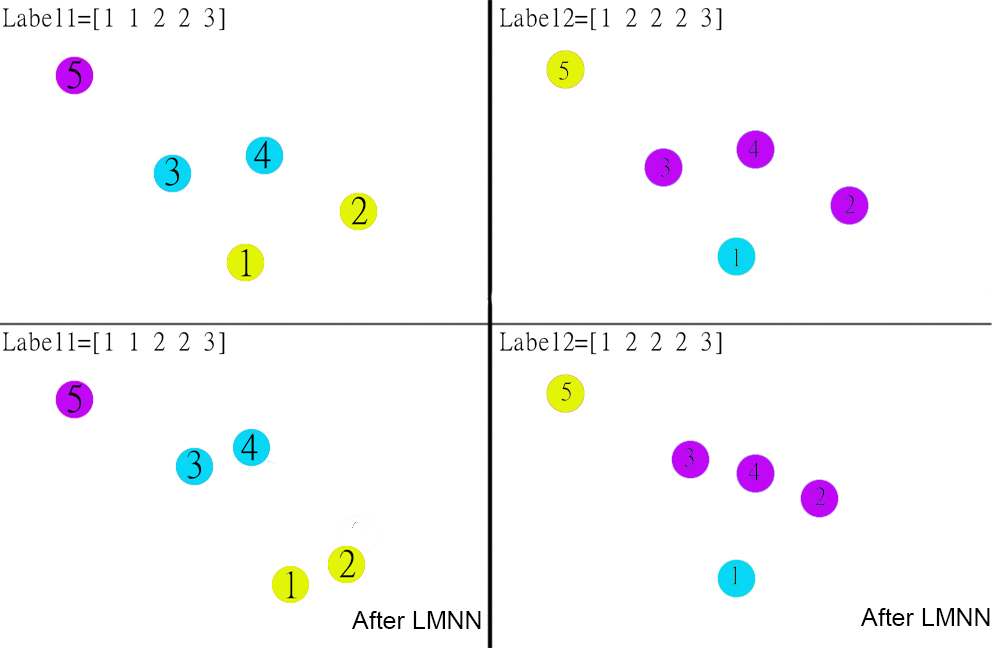
\includegraphics[width=1\textwidth]{lmnnex1}
    \caption{LMNN applied on two different labeling opinion}
    \label{Lmnnsum}
\end{figure}

\begin{enumerate}
\item The two labeling opinion agrees on the similarity.\\
The application of LMNN will conduct to a smaller distance if the labels are similar. If the observations are target neighbors both distances will be smaller in the new space for both labeling provided by the two different users. Observation 3 and 4 in figure 1 illustrate that idea. In this case the two distances $D_{M_1}$ and $D_{M_2}$ will be smaller than the original distance in the space before the application of LMNN. Let us now go back to update our new pair wise distance matrix: 
$$D_{M_1}34<d_{34}\  and \  D_{M_2}34<d_{34} $$ the sum of those two terms is thus : $$D_{M_1}34+D_{M_2}34<2d_{34}$$.
\item The two labeling opinion agrees on the non similarity.\\
The same analogy can be made for the case were both opinion agree that the two observation belongs to different classes. If we take for example the observations 1 and 3 we will have at the end  $$D_{M_1}34+D_{M_2}34>2d_{34}$$.
\item The two labeling opinion dos not agrees on the similarity.\\
If the two labeling opinion disagree on the similarity between two observation, in one space we will have smaller distance while in the second we will have bigger distance. For example if we look at samples  2 and 4 in figure 1, we can see that in the new spaces distance between those two observations is bigger for the new space with LMNN based on labeling opinion 1, and bigger in the space with LMNN based on labeling opinion 2. we will thus have : $$D_{M_1}24>d_{24} \ and \ D_{M_2}24<d_{24}$$. Let us introduce two factors $\alpha>1$ and $\beta<1$ this implies : $$D_{M_1}24=\alpha d_{24}\ and \ D_{M_2}24=\beta d_{24}$$
$$D_{sum}24=\alpha d_{24}+\beta d_{24}$$. 
\item An observation is not affected in both spaces by LMNN.\\
If the distance between two observations that are not target neighbors for the LMNN is bigger than a certain margin the distance will not be affected directly. This distance will slightly change because the observation themselves have been displaced in their own small margin. We can thus make the assumption that the variation in distance in the new space is negligible and the for example the distance between observation 1 and 5 will be $$D_{sum}15=2d_{15}$$
\end{enumerate}
Now that we have formulated all the factors we can construct our new matrix based on the sum of the projection matrix L. To simplify the notation we will take on factor to represent the different factors in case 3, for example let $2A=\alpha+\beta$.
\[
\begin{bmatrix}
1            & 2Ad_{12} & >2d_{13}  & >2d_{14} & 2d_{15} \\
2Ad_{21}     & 1        & 2Cd_{23}  & 2Bd_{24} & 2d_{25} \\
>2d_{31}     & 2Cd_{32} & 1         & <2d_{34} & 2d_{35} \\
>2d_{41}     & 2Bd_{42} & <2d_{43}  & 1        & 2d_{45} \\
2d_{51}      & 2d_{52}  & 2d_{53}   & 2d_{54}  & 1
\end{bmatrix}
\]
Let us now examine two cases, one where we have an agreement and one were we have a disagreement :
\begin{enumerate}
\item Case were we have agreement between different opinions.\\
It should be noted again that we are searching to compare distances and not the exact value of the distances. So let us take two distances were in the first both users agree that two samples belongs to the same class and in the other they agree that they don't.  for example we can take $d_{13} \ and \ d_{34}$. In the space before the application of LMNN we had : $d_{13}-d_{34}$ in the new space we will have a difference between a value that is twice bigger than the first distance and a value that is twice smaller than the second distance. So we have been able to have a space that make the difference in distances bigger if we have two exact opinions on labeling. And for both labeling opinions the error will be minimized.
\item Case were we have disagreement between opinions.
Let us take again distance $d_13$ but this time let us compare it with $d_21$. Let us take F as a value that is bigger than 1 to represent the factor by which in the new space the distance between samples 1 and 3 is bigger. we will thus have in the new space $2Fd_{13}-2Ad_{d21}$. We now that the first distance is going to be bigger than the original distance between samples 1 and 2. On the other hand the distance between 1 and 2 in the new space will depend on the original distance between 1 and 2. So if the distance in the new space is smaller than in the original space, labeling based on first user will have smaller error than labeling based on second user. But since the first factor is well optimized we will have optimization in both case. \\
This idea that the "winner" between the two opinion is based on the representation in the original space is very important. And it will be essential in a case were we have more than two opinions, since the probability that two samples will be considered similar by the users is related to the physical aspect of the sound. 
 \end{enumerate}
 \item \textbf{Weighting the sum over distances} \par 
In this case, the sum is weighted based on a factor of relevance of each labeling opinion relatively to the other labeling opinions. The success is based on a precision factor obtained by applying the normalized mutual information (NMI) \cite{K03}. The distances is thus  multiplied each one by the precision of the labeling opinion over the entire labeling opinion space. The results are as follows :
\begin{table} [H]
\begin{center} 
\ 
 \setlength{\tabcolsep}{.16667em} 
\begin{tabular}{ | l | l | l | l | l | l |}
\hline
features & MAP & MAP after LMNN & P@5 & p@5 after LMNN  \\ 
\hline 
mfcc & 50.74& 54.35 & 55.66 & 60.51  \\ 
scattering & 40.17 & 52.61 & 44.01 & 66.89   \\
\hline Case of taking all the sound pitch :
\\
\hline
mfcc  & 34.96  & 36.10 & 81.28  & 82.25 \\
scattering & 30.84  & 31.32 & 54.02  & 65.90 \\

\hline
\end{tabular} 
\end{center} 
\caption{Results of weigthing the sum} 
\label{you} 
\end{table} 
 
 weigthing the distance provides a small improvements over non weighted results. For the MFCC the effect is minimal whether for the scattering it provides improvement of around 1\%.
 
\item \textbf{Normalizing the distance}\par 
In this method, the distances has been normalized before performing the sum. This is to reduce the effect of big distances provided by one user over small distances provided by the rest for the same two observations. The results are presented in the following table :
\begin{table} [H]
\begin{center} 
\ 
 \setlength{\tabcolsep}{.16667em} 
\begin{tabular}{ | l | l | l | l | l | l | l |}
\hline
features & metrics & MAP & MAP +LMNN & P@5 & P@5 + LMNN  \\ 
\hline 
mfcc & normalized distance sum & 50.74 & 54.31 & 55.66 & 60.29  \\ 
mfcc & normalized w. distance sum &50.74 & 54.39 & 55.66 & 60.09  \\ 
scattering & normalized distance sum & 40.17 & 54.03 & 44.01 & 67.33  \\ 
scattering & normalized w. distance sum  & 40.17 & 54.30 & 44.01 & 67.63 \\
\hline All the sound pitch :
\\
\hline 
mfcc & normalized distance sum & 34.96  & 36.16 & 81.28  & 82.24 \\ 
mfcc & normalized w. distance sum & 34.96 & 36.15 & 81.28 & 82.27 \\ 
scattering & normalized distance sum & 30.84 & 31.32 & 54.02 & 65.56  \\ 
scattering & normalized w. distance sum  & 30.84  & 31.31 & 54.02  & 65.85  \\
\hline
\end{tabular} 
\end{center} 
\caption{Results of normalizing the distances} 
\label{you} 
\end{table}  
 Normalizing before effecting the sum proved to be beneficial for the scattering and not for the MFCC. This is due to the high conventionality of the scattering that might have an affect over the distances. This effect will be reduced by applying a normalization over the distances.
 \item \textbf{Class Matching} \par 
 The last method that was tested is to apply a class matching over the space of different observation. This is done using the NMI(normalized mutual information) technique. After matching the space of opinions, all the classes will are aligned. Now using a majority vote over the space of observations, only one set of labels is obtained. The LMNN will be thus trained only once on the obtained labeling. This will induce a shorter amount of training time and a faster algorithm. The results are given in the following table : 
 \begin{table}[H] 
\begin{center} 
\ 
 \setlength{\tabcolsep}{.16667em} 
\begin{tabular}{ | l | l | l | l | l | l |}
\hline
features & map & mapafter & pat5 & pat5after\\ 
\hline 
mfcc & 50.74 & 55.34 & 55.66 & 61.77 \\ 
scattering & 40.17 & 49.41 & 44.01 & 60.75  \\  

\hline All the sound pitch :
\\
\hline
mfcc & 34.96 & 35.77 & 81.28 & 81.99 \\ 
scattering & 30.84  & 31.14 & 54.02 & 67.74 \\  
\hline
\end{tabular} 
\end{center} 
\caption{Results of applying class matching before using LMNN} 
\label{you} 
\end{table}  
The class matching proves to be beneficial for the MFCC over the sum of distances. For the scattering summing the distances is better but with dramatically more computation time : For the class matching 21.01 seconds and for the sum of distances 2316.59 seconds.  
\end{enumerate}

\section{Conclusion}
This paper provided a study of two problems of music search query. The first one based on the physical aspect of the sound. The results obtained for this part and the preprocessing technique for the scattering are novel work. The precision obtained on the search query for musical purposes proved that the standard deviation of the scattering should be studied in order to achieve state of the art results. This technique of preprocessing should be tested for different problems in the domain of audio and images.
In the second part, the problem of studying multiple user opinion in order to find a space that respects all the opinions was addressed. This novel work has studied interesting research avenues for solving the problem.

\newpage
\begin{thebibliography}{2}
\bibitem{B00} 
Beth Logan
\textit{Mel Frequency Cepstral Coefficients for Music Modeling}. 
2000

\bibitem{AM11} 
J. Andén and S. Mallat. 
\textit{Multiscale scattering for audio classification.}. 
ISMIR 2011

\bibitem{A14} 
J. Andén 
\textit{Time and frequency scattering for audio classification}. 
January 7, 2014

\bibitem{H95}
Hermann Ludwig Ferdinand von Helmholtz
\textit{On the sensations of tone as a physiological basis}.
1895

\bibitem{M10}
Stephan Mallat 
\textit{Recursive interferometric Representations}  18th European Signal Processing Conference 2010
\bibitem{P03}
Perfecto Herrera-Boyer and al.
\textit{Automatic Classification of Musical Instrument Sounds}.
Journal of New Music Research 2003


\bibitem{SOL}
Yan Maresz and al.
\textit{Ircam solo instruments UltimateSoundBank reference guide}

\bibitem{W09}
K. Q. Weinberger, L. K. Saul. 
\textit{Distance Metric Learning for Large Margin Nearest Neighbor Classification}.
Journal of Machine Learning Research (JMLR) 2009

\bibitem{X02}
P. Xing, A. Y. Ng, M. I. Jordan, and S. Russell 
\textit{Distance metric learning, with application to
clustering with side-information}.
 Cambridge, MA, 2002.
 \bibitem{S04}
 Shalev-Shwartz, Y. Singer, and A. Y. Ng.
 \textit{Online and batch learning of pseudo-metrics}
 Banff, Canada, 2004.
 \bibitem{G05}
 Goldberger, S. Roweis, G. Hinton, and R. Salakhutdinov.
 \textit{Neighbourhood components analysis}
 Cambridge, MA, 2005
 
 \bibitem{K03}
  Kraskov Alexande and al. ,
  \textit{Hierarchical Clustering Based on Mutual Information}
  Grassberger, Peter (2003)
\end{thebibliography}
\end{document}